\chapter{Implementacja logiki symulacji}
 Niniejszy rozdział skupia się na implementacji zasad fizyki orbitalnej, systemie zarządzania czasem oraz mechanizmach interakcji użytkownika z wirtualnym Układem Słonecznym.

    % 5.1
    \section{Fizyka i model danych ciał niebieskich (\file{r\_physics})}
     Model fizyczny aplikacji został zaprojektowany w oparciu o uproszczoną mechanikę nieba, wykorzystującą parametry orbitalne do deterministycznego wyznaczania pozycji ciał niebieskich w dowolnym momencie czasu.

        % 5.1.1
        \subsection{Struktura planety (\file{planet\_t})}

         \begin{itemize}
             \item[---] \textbf{Dane identyfikacyjne i wizualne:} Nazwa planety (\var{name}) oraz kolor bazowy (\var{color}) wykorzystywany przez elementy interfejsu.
             \item[---] \textbf{Elementy orbitalne Keplera:}
             \begin{itemize}
                 \item[---] \var{orbit.semi_major_axis}: Średnia odległość od ciała centralnego
                 \item[---] \var{orbit.period_orbital}: Czas pełnego obiegu wokół orbity (rok gwiazdowy)
                 \item[---] \var{orbit.mean_anomaly_epoch}: Przesunięcie początkowe, pozwalające ustalić pozycję planety w epoce startowej (np. J2000)
                 \item[---] \var{inclination}: Kąt nachylenia płaszczyzny orbity do płaszczyzny odniesienia (ekliptyki)
                 \item[---] \var{long_asc_node}: Kąt określający orientację orbity w płaszczyźnie odniesienia
             \end{itemize}
             \item[---] \textbf{Parametry rotacyjne:} \var{period_rotation} (okres obrotu wokół własnej osi) oraz \var{obliquity} (nachylenie osi obrotu).
             \item[---] \textbf{Hierarchia:} Wskaźnik \var{struct planet *parent}, umożliwiający tworzenie układów zależnych (np. Księżyc krążący wokół Ziemi, która krąży wokół Słońca).
         \end{itemize}

         \newpage

        % Rysunek 5.1 Schemat "Elementy orbitalne Keplera"

        \vspace{1em}
        \begin{table}[htpb]
        \centering
        \caption{Wybrane parametry fizyczne i orbitalne ciał niebieskich zaimplementowane w kodzie symulacji}
        \label{tab:planets_data}
        \resizebox{\textwidth}{!}{% Skalowanie tabeli do szerokości strony
        \begin{tabular}{|l|r|r|r|r|r|}
        \hline
        \textbf{Ciało niebieskie} & \textbf{Promień równikowy [km]} & \textbf{Półoś wielka [km]} & \textbf{Mimośród} & \textbf{Okres orbitalny [dni]} & \textbf{Inklinacja [$^\circ$]} \\ \hline
        Słońce  & 695 700.0 & 0.0         & 0.000000 & 0.0     & 0.000  \\ \hline
        Merkury & 2 439.7   & 57 909 227  & 0.205630 & 87.97   & 7.005  \\ \hline
        Wenus   & 6 051.8   & 108 209 475 & 0.006772 & 224.70  & 3.395  \\ \hline
        Ziemia  & 6 371.0   & 149 597 870 & 0.016708 & 365.26  & 0.000  \\ \hline
        Mars    & 3 389.5   & 227 939 200 & 0.093400 & 686.98  & 1.850  \\ \hline
        Jowisz  & 69 911.0  & 778 340 821 & 0.048498 & 4332.59 & 1.304  \\ \hline
        Saturn  & 58 232.0  & 1 426 666 422 & 0.055546 & 10759.22& 2.485  \\ \hline
        Uran    & 25 362.0  & 2 870 658 186 & 0.047318 & 30685.40& 0.773  \\ \hline
        Neptun  & 24 622.0  & 4 498 396 441 & 0.008606 & 60189.00& 1.770  \\ \hline
        Pluton  & 1 188.3   & 5 906 380 000 & 0.248800 & 90560.00& 17.160 \\ \hline
        \end{tabular}%
        }
        \end{table}

        % 5.1.2
        \subsection{Integracja z grafiką}
         Kluczowym aspektem architektury jest sposób połączenia warstwy fizycznej z warstwą prezentacji.
         Zamiast dziedziczenia, zastosowano kompozycję: struktura \var{planet\_t} zawiera wskaźnik \var{object\_t *object}.
        
         Obiekt graficzny (\var{object\_t}) przechowuje siatkę geometryczną, teksturę i shader, ale nie posiada wiedzy o swojej pozycji w kontekście astronomicznym.
         W każdej klatce symulacji, funkcja aktualizująca stan planety oblicza nową pozycję, a następnie modyfikuje macierz modelu (\var{u_Model}) powiązanego obiektu graficznego.

         Dzięki temu rozwiązaniu, renderer pozostaje niezależnym modułem, który jedynie "wyświetla" to, co obliczyła fizyka.
         Pozwala to również na łatwą zmianę reprezentacji wizualnej planety (np. podmianę modelu na dokładniejszy) bez ingerencji w kod fizyki.

         \newpage

        \vspace{1em}
        \begin{lstlisting}[language=C, caption={Budowa finalnej macierzy modelu w pętli głównej poprzez sekwencyjne nakładanie transformacji: nachylenia osi (obliquity), rotacji dobowej, skalowania oraz pozycji orbitalnej}, label={lst:model_matrix}]
    mat4_t model = mat4(1.0f);

    // Aplikacja nachylenia osi i rotacji planety
    model = r_rotate(model, context.scene.planets[i].obliquity * (180.0f / R_PI), vec3(0.0f, 0.0f, 1.0f));
    model = r_rotate(model, context.scene.planets[i].state.rotation * (180.0f / R_PI), vec3(0.0f, 1.0f, 0.0f));

    // Aplikacja skali fizycznej
    float scale = (i == 0) ? 0.8f : 1.6f;
    model = r_scale(model, vec3_mul(vec3(
        context.scene.planets[i].radius_equatorial * scale, 
        context.scene.planets[i].radius_equatorial * scale, 
        context.scene.planets[i].radius_equatorial * scale
    ), R_PHYSICS_PLANET_SCALE));

    // Aplikacja pozycji orbitalnej z przestrzeni r_physics
    model = r_translate(model, vec3_mul(context.scene.planets[i].state.position, R_PHYSICS_ORBIT_SCALE));

    r_set_mat4(context.scene.planets[i].object -> shader, "u_Model", model);
        \end{lstlisting}

         \newpage

        % 5.1.3
        \subsection{Algorytm pozycyjny}
         Wyznaczanie pozycji ciał niebieskich realizowane jest przez funkcję \func{r\_physics\_planet\_state\_update} oraz pomocniczą funkcję \func{r\_physics\_orbit\_to\_local}. 
         Proces ten przebiega w następujących krokach:

         \begin{enumerate}
             \item \textbf{Obliczenie anomalii średniej:} Na podstawie aktualnego czasu symulacji (\var{time}) wyznaczany jest kąt na orbicie (\var{orbit\_angle}). Uwzględnia się przy tym okres orbitalny oraz fazę początkową.
             \item \textbf{Wyznaczenie pozycji na płaszczyźnie orbity:} Współrzędne obliczane są przy założeniu orbity kołowej (dla uproszczenia mimośrodów bliskich zeru):
                 \begin{equation}
                 x = r \cdot \cos(\theta), \quad z = r \cdot \sin(\theta)
                 \end{equation}
             \item \textbf{Transformacja do układu lokalnego:} Pozycja jest poddawana obrotom zgodnie z parametrami orbitalnymi. Najpierw następuje obrót o kąt inklinacji wokół osi X, a następnie obrót o kąt węzła wstępującego wokół osi Y.
             \item \textbf{Uwzględnienie hierarchii:} Jeśli planeta posiada rodzica (pole parent nie jest NULL), do obliczonej pozycji dodawany jest wektor pozycji rodzica. Pozwala to na poprawne symulowanie układów satelitarnych.
         \end{enumerate}

         \newpage

         \textbf{Algorytm Newtona-Raphsona}
         
         \bigbreak

         Podstawowym wyzwaniem w modelu keplerowskim jest wyznaczenie anomalii mimośrodowej ($E$) na podstawie anomalii średniej ($M$) oraz mimośrodu orbity ($e$).
         Zależność tę opisuje równanie Keplera:

         \begin{equation}
         M = E - e * \sin(E)
         \end{equation}

         Równanie to jest równaniem przestępnym i nie posiada jawnego rozwiązania analitycznego.
         W celu jego rozwiązania w czasie rzeczywistym, w module fizycznym (\func{\_r\_physics\_kepler\_solve}) zaimplementowano numeryczną metodę Newtona-Raphsona.
         W kolejnych iteracjach pętli, przybliżona wartość $E$ jest korygowana zgodnie ze wzorem:

         \begin{equation}
         E_{n+1} = E_n - \frac{E_n - e \sin(E_n) - M}{1 - e \cos(E_n)}
         \end{equation}

         Dzięki bardzo szybkiemu tempu zbieżności tej metody, wystarczy zaledwie kilka iteracji (w implementacji założono stałą liczbę 5 kroków), aby uzyskać precyzję zmiennoprzecinkową wystarczającą dla poprawnego i płynnego pozycjonowania ciał niebieskich na orbitach.

        \vspace{1em}
        \begin{lstlisting}[language=C, caption={Implementacja algorytmu Newtona-Raphsona do numerycznego rozwiązywania równania Keplera}, label={lst:kepler_solve}]
        double _r_physics_kepler_solve(double mean, double eccentric) {
            double E = mean;
            for (uint32_t i = 0; i < 5; i++) {
                double delta = E - eccentric * sin(E) - mean;
                E = E - delta / (1.0 - eccentric * cos(E));
            }
            return E;
        }
        \end{lstlisting}

        \newpage

    % 5.2
    \section{System czasu i kalendarza}
     Zarządzanie czasem jest krytycznym elementem symulacji astronomicznej, pozwalającym na obserwację zjawisk zachodzących w skali od minut do stuleci.

        % 5.2.1
        \subsection{Obsługa czasu rzeczywistego i symulowanego}
         Wewnętrzny zegar symulacji (\var{context.scene.clock.time}) reprezentowany jest przez zmienną typu double, przechowującą liczbę sekund, jakie upłynęły od epoki J2000 (1 stycznia 2000, 12:00 TT).
         Taka reprezentacja zapewnia wysoką precyzję i ułatwia obliczenia astronomiczne.

         W celu prezentacji daty użytkownikowi, zaimplementowano funkcję \func{r\_physics\_clock\_to\_tm}, która konwertuje czas liniowy na strukturę kalendarzową \var{struct tm} (rok, miesiąc, dzień).
         Wykorzystano w tym celu standardowe funkcje biblioteki C (\var{mktime, localtime_r}), traktując rok 2000 jako punkt odniesienia.

        % 5.2.2
        \subsection{Mechanizm sterowania upływem czasu}
         Aplikacja umożliwia dynamiczną zmianę prędkości upływu czasu. 
         Zaimplementowano to przy użyciu tablicy prędkości \var{speeds} oraz kursora wskazującego na aktualnie wybrany mnożnik. 
         Tablica zawiera wartości od ujemnych (cofanie czasu), przez zero (pauza), aż po wartości dodatnie symulujące upływ lat w ciągu sekund.

         W każdej klatce pętli głównej, czas symulacji jest inkrementowany o wartość: \var{context.fps.time_between_frames} * \var{speeds[cursor]}.
         
         Sterowanie odbywa się za pomocą klawiszy klawiatury (H - zwolnienie/cofanie, K - przyspieszenie, J - reset do czasu rzeczywistego), co pozwala użytkownikowi na płynną nawigację w chronologii Układu Słonecznego.

        \vspace{1em}
        \begin{table}[htpb]
        \centering
        \caption{Skróty klawiszowe umożliwiające manipulację kalendarzem symulacji}
        \label{tab:time_controls}
        \begin{tabular}{|c|p{10cm}|}
        \hline
        \textbf{Klawisz} & \textbf{Akcja (zmiana w tablicy \var{speeds})} \\ \hline
        \textbf{H} & Zmniejszenie mnożnika upływu czasu (pozwala na zwolnienie biegu wydarzeń, zatrzymanie, aż do płynnego cofania symulacji). \\ \hline
        \textbf{K} & Zwiększenie mnożnika upływu czasu (przyspieszenie symulacji, pozwalające zaobserwować ruch powolnych planet zewnętrznych). \\ \hline
        \textbf{J} & Błyskawiczny reset wskaźnika (\var{cursor = 17}) do domyślnego upływu czasu. \\ \hline
        \end{tabular}
        \end{table}

        \vspace{1em}
        \begin{table}[htpb]
        \centering
        \caption{Pełne zestawienie dostępnych mnożników upływu czasu (wartości tablicy \var{speeds}), po których porusza się kursor sterowania}
        \label{tab:time_speeds}
        \begin{tabular}{|c|l|l|}
        \hline
        \textbf{Indeks (kursor)} & \textbf{Upływ czasu w grze (na 1 sekundę rzeczywistą)} & \textbf{Reprezentacja w kodzie symulacji} \\ \hline
        0  & $-1$ rok (szybkie cofanie) & \var{-R\_PHYSICS\_YEAR\_SECONDS} \\ \hline
        1  & $-10$ miesięcy             & \var{-10 * R\_PHYSICS\_MONTH\_SECONDS} \\ \hline
        2  & $-1$ miesiąc               & \var{-R\_PHYSICS\_MONTH\_SECONDS} \\ \hline
        3  & $-10$ dni                  & \var{-10 * R\_PHYSICS\_DAY\_SECONDS} \\ \hline
        4  & $-1$ dzień                 & \var{-R\_PHYSICS\_DAY\_SECONDS} \\ \hline
        5  & $-10$ godzin               & \var{-10 * R\_PHYSICS\_HOUR\_SECONDS} \\ \hline
        6  & $-1$ godzina               & \var{-R\_PHYSICS\_HOUR\_SECONDS} \\ \hline
        7  & $-10$ minut                & \var{-10 * R\_PHYSICS\_MINUTE\_SECONDS} \\ \hline
        8  & $-1$ minuta                & \var{-R\_PHYSICS\_MINUTE\_SECONDS} \\ \hline
        9  & $-10$ sekund               & \var{-10.0} \\ \hline
        10 & $-1$ sekunda (czas wstecz) & \var{-1.0} \\ \hline
        11 & $1$ sekunda (czas realny)  & \var{1.0} \\ \hline
        12 & $10$ sekund                & \var{10.0} \\ \hline
        13 & $1$ minuta                 & \var{R\_PHYSICS\_MINUTE\_SECONDS} \\ \hline
        14 & $10$ minut                 & \var{10 * R\_PHYSICS\_MINUTE\_SECONDS} \\ \hline
        15 & $1$ godzina                & \var{R\_PHYSICS\_HOUR\_SECONDS} \\ \hline
        16 & $10$ godzin                & \var{10 * R\_PHYSICS\_HOUR\_SECONDS} \\ \hline
        \textbf{17} & \textbf{1 dzień (domyślny startowy)} & \textbf{\var{R\_PHYSICS\_DAY\_SECONDS}} \\ \hline
        18 & $10$ dni                   & \var{10 * R\_PHYSICS\_DAY\_SECONDS} \\ \hline
        19 & $1$ miesiąc                & \var{R\_PHYSICS\_MONTH\_SECONDS} \\ \hline
        20 & $10$ miesięcy              & \var{10 * R\_PHYSICS\_MONTH\_SECONDS} \\ \hline
        21 & $1$ rok (szybkie przewijanie) & \var{R\_PHYSICS\_YEAR\_SECONDS} \\ \hline
        \end{tabular}
        \end{table}

    % 5.3
    \section{Interfejs i interakcja w przestrzeni 3D}
     Ze względu na specyficzną skalę kosmosu (ogromne odległości i stosunkowo małe obiekty), konieczne było zaprojektowanie elementów wizualnych ułatwiających orientację w przestrzeni.

        % 5.3.1
        \subsection{Wizualizacja orbit}
         Linie orbit nie są częścią modeli 3D, lecz są generowane proceduralnie podczas inicjalizacji sceny (\func{\_g\_game\_ui\_orbits\_init}). 
         Algorytm iteruje przez kąt od $0$ do $2\pi$ z zadanym krokiem, wykorzystując tę samą funkcję fizyczną \func{r\_physics\_orbit\_to\_local}, która służy do pozycjonowania planet.

         Wygenerowane wierzchołki są przesyłane do osobnego bufora VBO i rysowane jako prymityw \var{GL_LINE_LOOP}. 
         Dzięki temu orbity idealnie pokrywają się z trajektorią ruchu planet, uwzględniając ich inklinację i ekscentryczność.
         Do ich renderowania użyto dedykowanego shadera (\file{orbit.vs}, \file{orbit.fs}), który umożliwia nadanie im stałego koloru i jasności, niezależnie od oświetlenia słonecznego. 

        \begin{figure}[htpb]
            \centering
            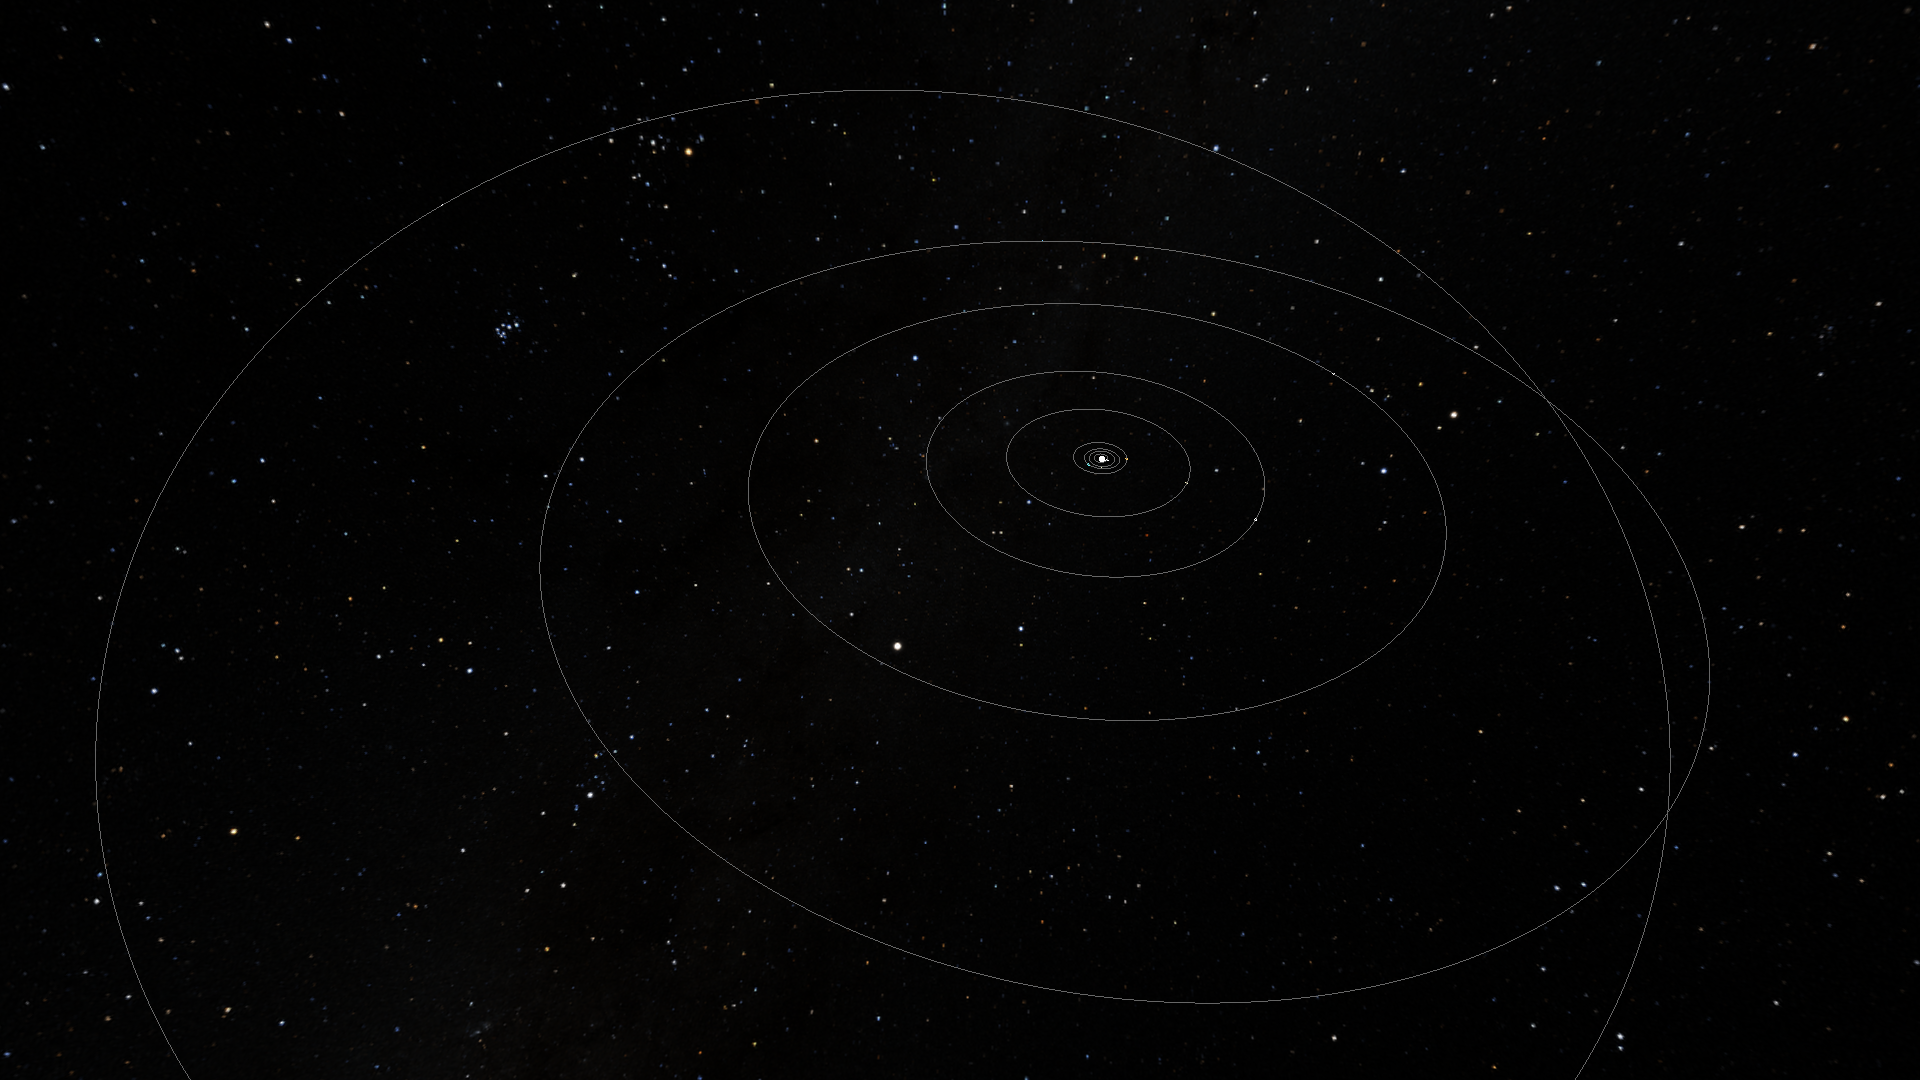
\includegraphics[width=0.95\textwidth]{images/orbits.png}
            \caption{Renderowanie proceduralnych linii orbit idealnie dopasowanych do wyliczonych matematycznie trajektorii planet}
            \label{fig:screen_orbits}
        \end{figure}

        \newpage

        % 5.3.2
        \subsection{System markerów i nawigacja}
         Aby planety były widoczne nawet z dużej odległości, zastosowano system markerów. 
         Są to proste okręgi rysowane wokół pozycji planety. 
         Marker jest skalowany w taki sposób, aby był zawsze zauważalny, ale skalowanie to odbywa się w shaderze lub poprzez macierz modelu markera (\var{model_marker}), która jest niezależna od skali samej planety.

         \bigbreak

         System nawigacji przestrzennej oparto na modelu swobodnej kamery (First Person Camera / Free Look). Znormalizowany wektor kierunku patrzenia wyznaczany jest w oparciu o klasyczne kąty Eulera: odchylenie (\var{yaw}) oraz pochylenie (\var{pitch}), których wartości są dynamicznie modyfikowane na podstawie przesunięć kursora myszy. Aby zapobiec zjawisku odwrócenia kamery i blokady przegubów (tzw. Gimbal Lock w osi pionowej), kąt pochylenia jest algorytmicznie ograniczany do przedziału $[-89^{\circ}, 89^{\circ}]$. 

         Następnie wektor orientacji bocznej (Right) oraz wektor pionu kamery (Up) wyliczane są za pomocą matematycznego iloczynu wektorowego (Cross Product) wektora kierunkowego i stałego wektora „góry” świata (\var{head\_position}). Translacja pozycji kamery odbywa się wzdłuż wyznaczonych w ten sposób wektorów lokalnych za pomocą klawiatury. Implementacja ta, zawarta w funkcjach \func{\_g\_game\_mouse\_handle} oraz \func{\_g\_game\_keyboard\_handle}, pozwala na intuicyjne przemieszczanie się po Układzie Słonecznym.

        % Rysunek 5.2 ""
        \begin{figure}[htpb]
            \centering
            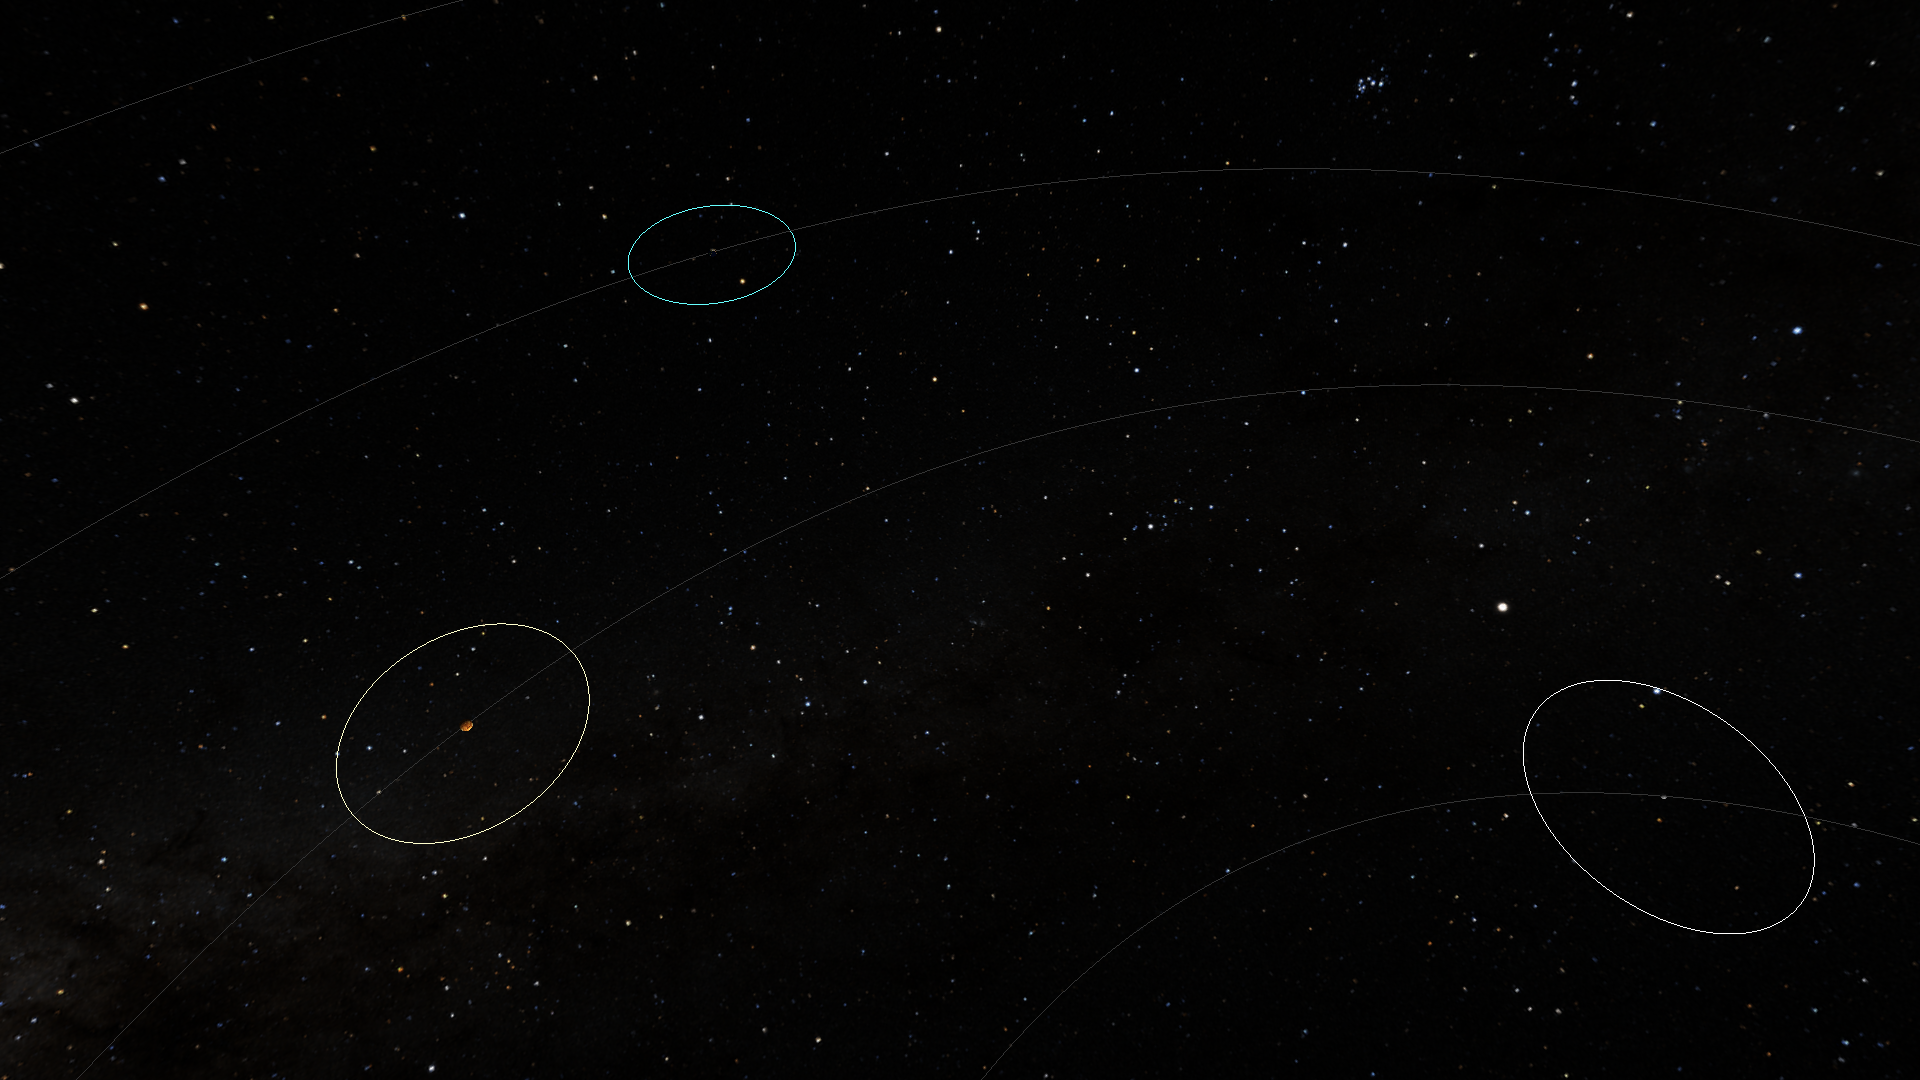
\includegraphics[width=0.95\textwidth]{images/markers.png}
            \caption{System skalowalnych markerów ułatwiający nawigację i lokalizację odległych obiektów w przestrzeni kosmicznej}
            \label{fig:screen_markers}
        \end{figure}
         